
\section{Modeling in Ptolemy}
\label{sec:modeling-ptolemy}

In this section, we present the strategy we followed to implement in Ptolemy the MAC layer of OpenWSN\footnote{Though the model in each figure is vector graphics, and it is possible to zoom in and read all the details, we  suggest the reader to open the attached Ptolemy model for further information}.

Our focus has been the modeling of the TSCH state machine. However, to obtain a runnable model we have also modeled a simple physical radio and abstracted the higher network layers as a single application layer. Figure~\ref{fig:OpenWSNNode} shows our stack of actors. We can see how the information flow proceed from the physical channel to the application layer and \emph{vice versa}. 

Taking a closer look, we defined each actor as follows:

{\bf PhysicalLayer:} This actor provides the interface to and from the physical channel and the rest of the network. Ports \texttt{fromPhysical}, \texttt{toPhysical}, \texttt{fromMAC} and \texttt{toMAC} are used to exchange data both during transmission and reception.
To simulate a realistic behavior, in which a packet needs a certain time to be received/sent, the \texttt{PhysicalLayer} actor adds delays whenever a packet needs to be forwarded in both directions. Ports \texttt{startOfFrame} and \texttt{endOfFrame} indicate to the MAC layer the beginning and the ending of a transmission/reception performed by the radio. 

{\bf AppLayer:} This actor represents the application that runs in each node. From a general point of view, the definition of the node behavior is this actor's responsibility. It communicates with the MAC layer through In this work, since our focus has been the MAC layer, we haven't implemented complex application models, leaving this task as a future work. \ai {I am not really sure about this paragraph}

\begin{figure*}[t]
\centering
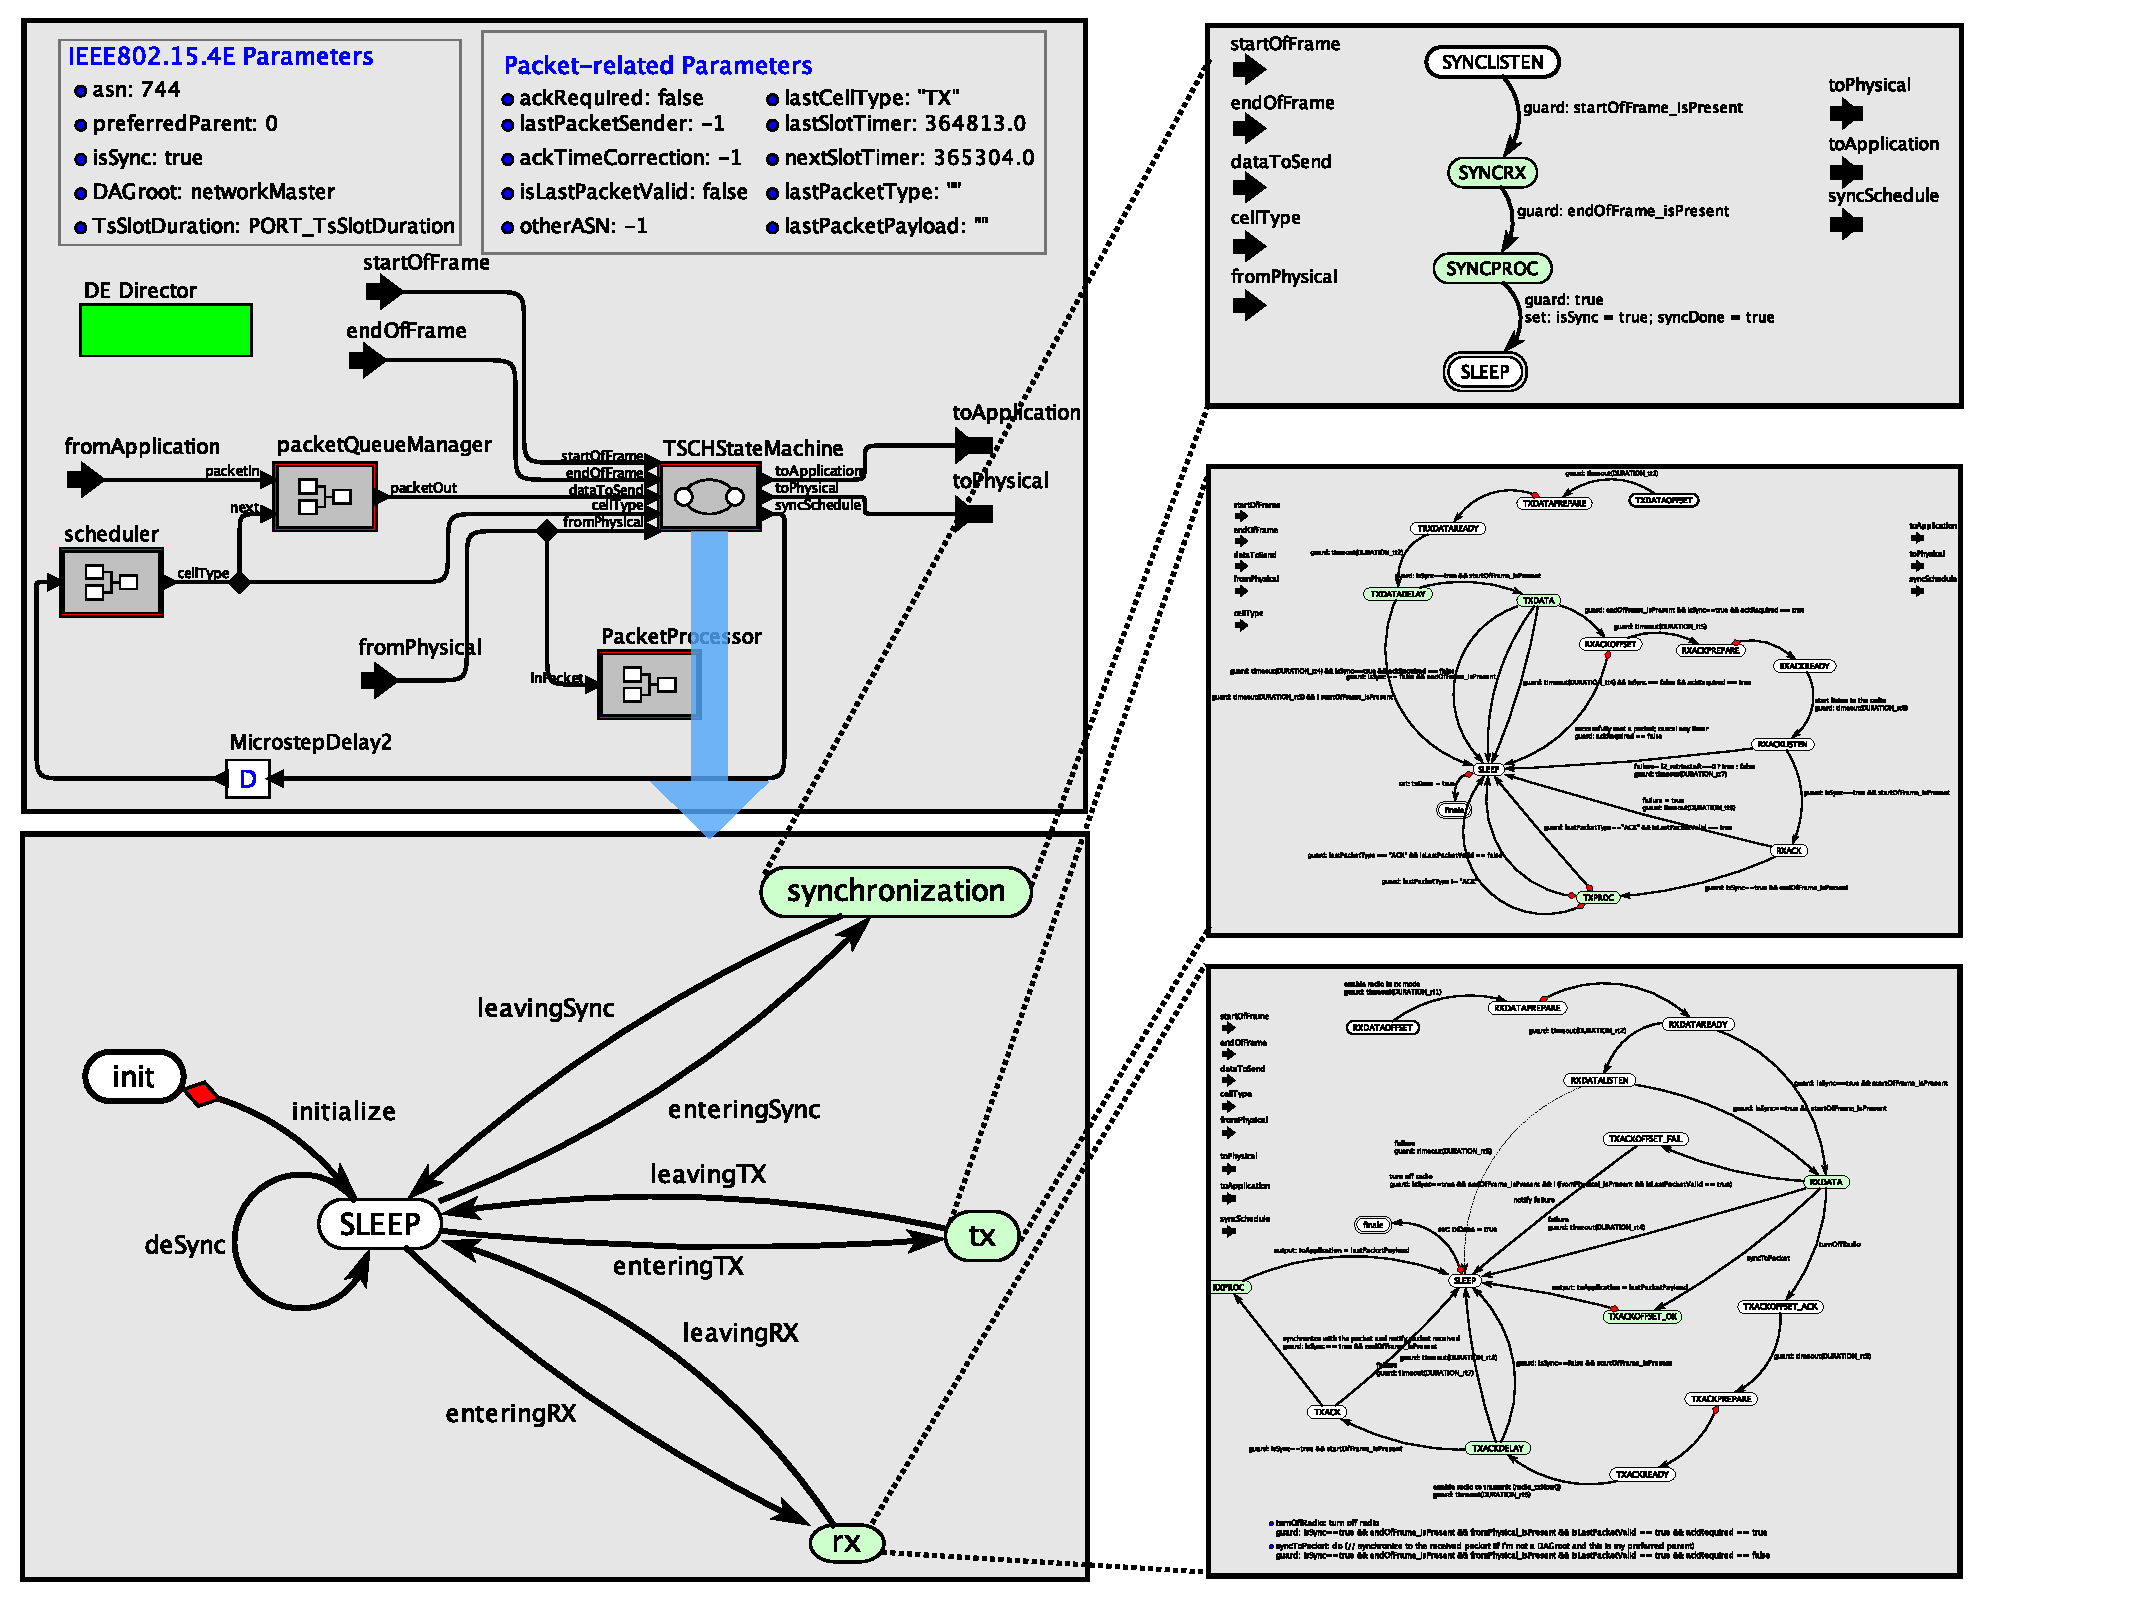
\includegraphics[width=\textwidth]{figures/PaperTSCHStateMachine}
\caption{The state machine with refinements of TSCH protocol.}
\label{fig:TSCHSM}
\end{figure*}

{\bf MACLayer:} In our model, this is the most important actor. Figure~\ref{fig:TSCHSM} gives an immediate yet detailed overview of its internal structure.
Actors \texttt{packetQueueManager} and \texttt{PacketProcessor} are used to handle packets coming from the application and the physical layers. In the first case, since the application sends packets arbitrarily, we need a queue system to store packets till the system is allowed to send them. In the second case, since a packet is received from the physical layer only when the MAC layer is in the reception phase, we just need an actor to extract information as the payload, the sender address, the validity of the packet, etc.
\texttt{scheduler} actor is responsible to communicate to the TSCH state machine what is the current slot ASN and when each slot starts. In our model, according to the actual OpenWSN implementation\footref{note:openWSN}, the schedule is predefined for each node. 

The \texttt{TSCHStateMachine} is implementated as a Ptolemy modal mode actor and consists of five main states, which describe the node activity: \texttt{init}, \texttt{SLEEP}, \texttt{synchronization}, \texttt{tx} and \texttt{rx}. 

During the initialization phase, all protocol related parameters are reset. When in the \texttt{synchronization} refinement, the node keeps listening for \texttt{ADV} packet and performs slot synchronization and ASN synchronization. Once the synchronization is done, it goes back to \texttt{SLEEP} state.
The scheduler decides node actions: 
\begin{itemize}
\item If the slot is \texttt{ADV} slot, then the node enters the \texttt{tx} state and sends an \texttt{ADV} packet. 
\item If it's \texttt{TX} or \texttt{RXTX} slot and the node has data to send (there are packets queued at \texttt{packetQueueManager}), it will enter \texttt{tx} state and send the data packet. 
\item If it's \texttt{RX} slot, or it's \texttt{RXTX} slot but the application doesn't have data to send, the node will enter \texttt{rx} state and listen for packets.
\end{itemize}

In both \texttt{tx} and \texttt{rx} states, there is a refinement which captures the complicated state transition of the radio. For example, when the node is sending a packet, it first wait a certain time (in \texttt{TXDATAOFFSET} state), then prepares the data for radio to transmit (\texttt{TXDATAPREPARE}), and after a few other states that are used to check the radio status, etc., it finally enters \texttt{TXDATA} state and transmits the packet. Similar complexity exists for managing acknowledgment and receiving a packet. Given our space constraints, we refer the reader to our Ptolemy model for more details on state transition behavior.

The \texttt{synchronization} state is only entered when the node is not synchronized to the rest of the network anymore. Additionally, for every received packet, the node will capture the reception time (Figure~\ref{fig:timeCorrection} {\em up}). If the packet is from a time master, it will calculate the time discrepancy and use it to adjust its synchronization (Figure~\ref{fig:timeCorrection} {\em middle}). If the packet is from a time slave, then the node will still perform a calculation and send the time correction through \texttt{ACK} packet (Figure~\ref{fig:timeCorrection} {\em down}).

\begin{figure}[t]
\centering
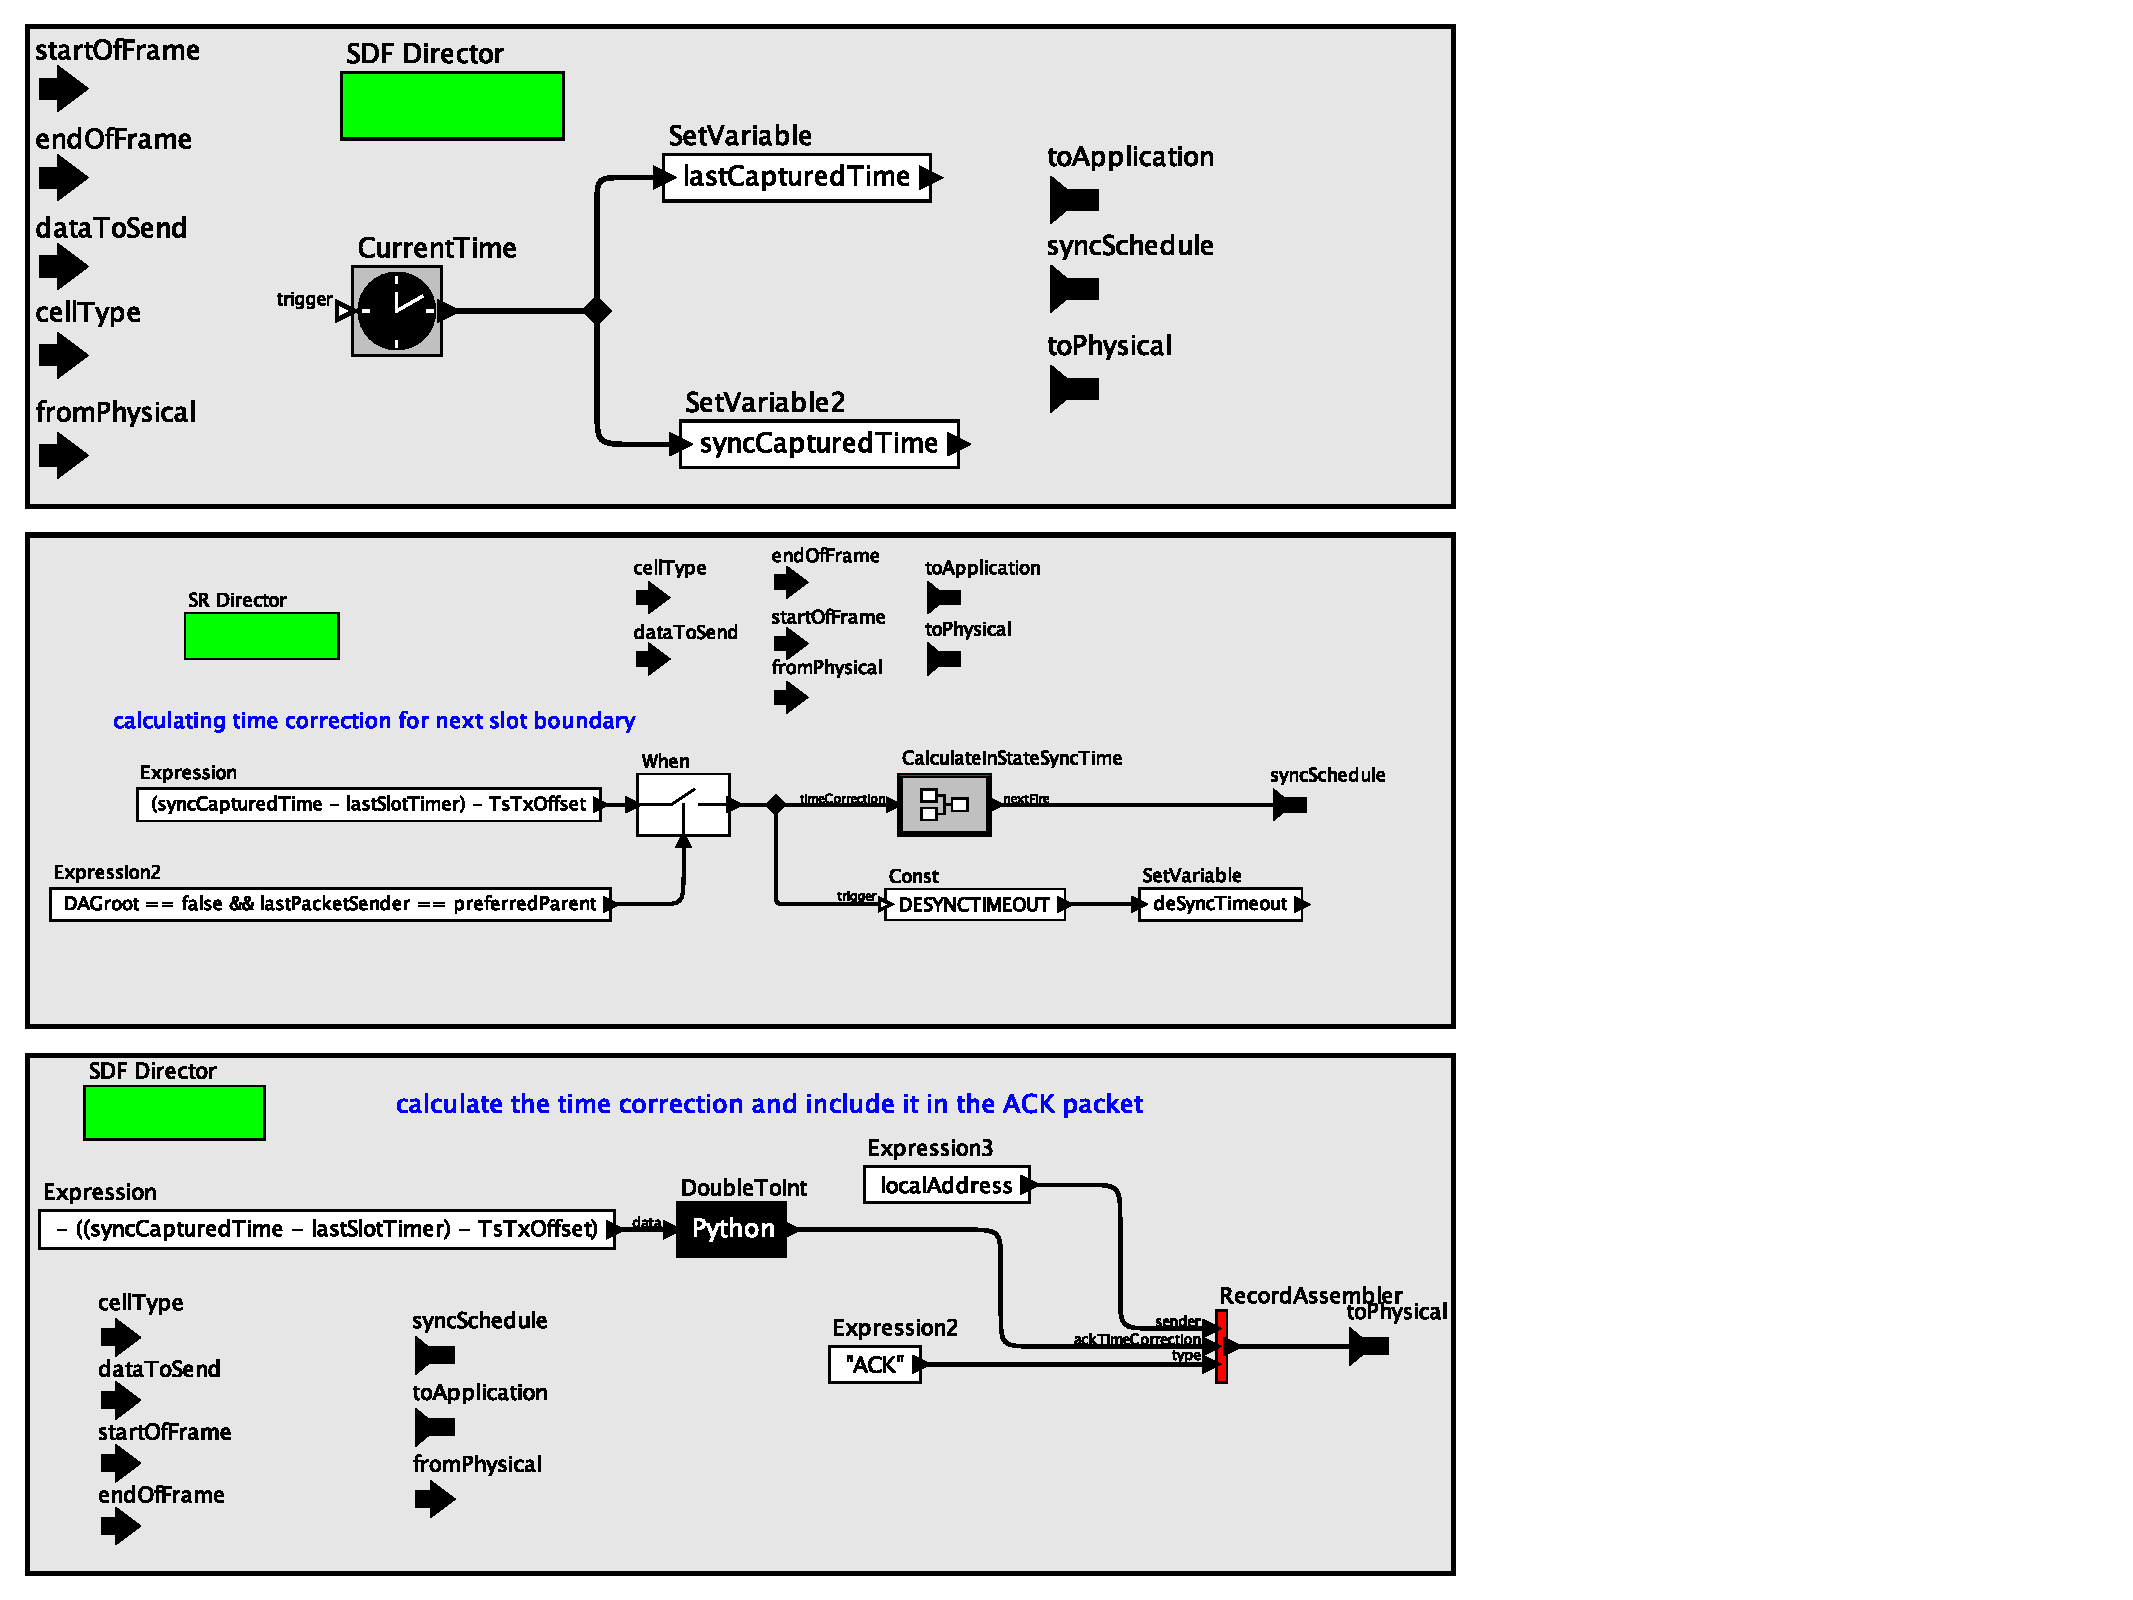
\includegraphics[width=0.9\columnwidth]{figures/PaperReSynchronization}
\caption{Modeling the the re-synchronization.}
\label{fig:timeCorrection}
\end{figure}


\subsection{Energy Consumption Modeling}
\label{sec:energy}


%%% Local Variables: 
%%% mode: latex
%%% TeX-master: "ee219d"
%%% End: 
